\section{Węzły torusowe} % (fold)
\label{sec:torus}
W tej sekcji przyjrzymy się węzłom o~specjalnym ułożeniu w~przestrzeni $\R^3$.
Do ich określenia potrzebny jest torus trywialny,
powierzchnia otrzymana przez obrót okręgu $(x-2)^2 + y^2 = 1$ wokół osi $y$.
Można go także uzyskać przez sklejenie podstaw walca tak, by go przy tym nie zapętlić.
Oczywiście istnieją też nietrywialne torusy, na przykład rurowe otoczenie trójlistnika.

\begin{definition}
    \index{węzeł!torusowy}
    Węzeł (splot) torusowy to taki, który leży na powierzchni niezaplątanego torusa.
\end{definition}

Na walcu $S^2 \times [0,1]$, którego podstawa leży w~płaszczyźnie $xy$, rozpatrzmy $r$ skierowanych odcinkach (dla $k = 0, 1, \ldots, r - 1$) o~końcach w~punktach
\begin{align*}
    \left(\cos \frac{2k \pi}{r}, \sin \frac{2k\pi}{r}, 0 \right), \quad
    \left(\cos \frac{2k \pi}{r}, \sin \frac{2k\pi}{r}, 1 \right).
\end{align*}
Przekręćmy górną podstawę walca wokół osi $z$ o~skierowany kąt $2\pi q / r$ oraz utożsammy ze sobą pary punktów $(x, y, 0) \sim (x, y, 1)$,
Uzyskaliśmy splot torusowy $K_{q, r}$: okrąża on $q$ razy rdzeń torusa i~$p$ razy jego oś symetrii obrotowej.
Określimy jeszcze kilka splotów torusowych.
Węzeł $K_{0, 0}$ leży na powierzchni torusa i~jest ściągalny do punktu, zaś $K_{1, 0}$ to nawinięta toroidalnie pętla.
Węzeł $K_{p, q}$ posiada następującą parametryzację:
\[
    x = (2+\cos q \phi) \cos p \phi, \quad
    y = (2+\cos q \phi) \sin p \phi, \quad
    z = - \sin q \phi, \quad
    0 \le \phi \le 2\pi.
\]
Poniżej przedstawiamy trzy węzły torusowe.

\begin{figure}[H]
    \begin{minipage}[b]{.3\linewidth}
        \centering
        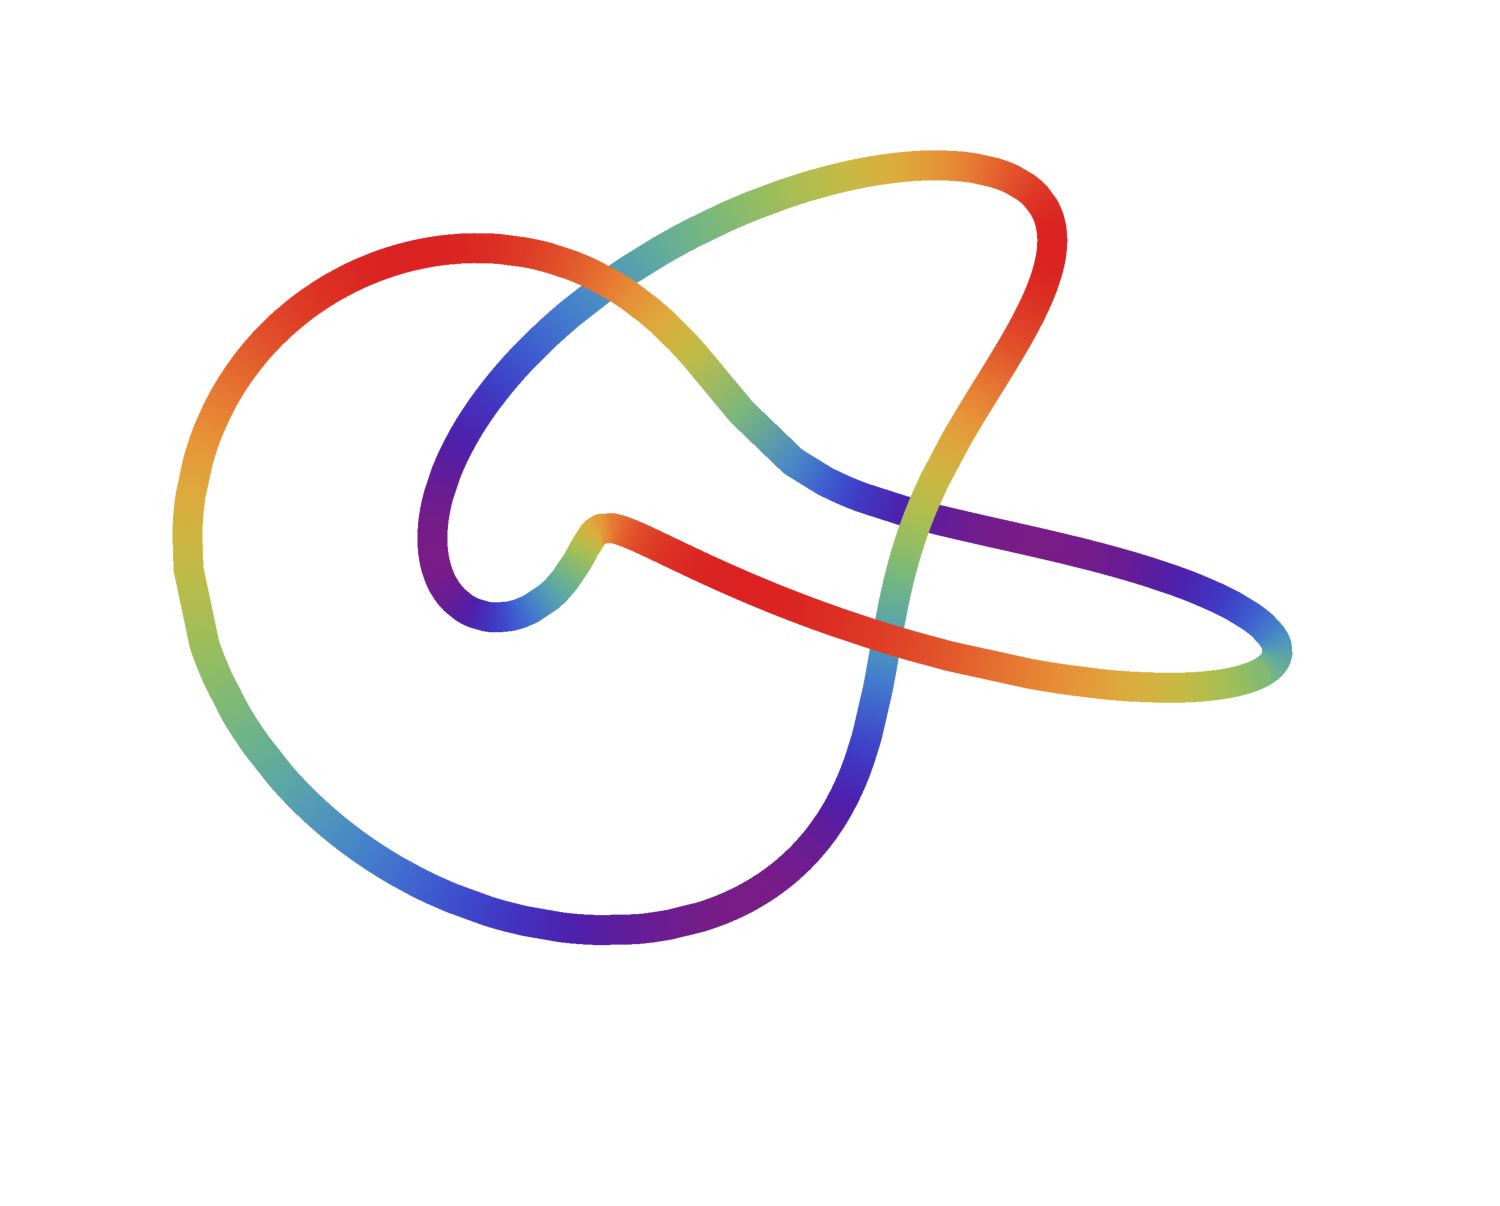
\includegraphics[width=\linewidth]{../data/torus-p2-q3.pdf}
        \subcaption{trójlistnik: $p = 2, q = 3$}
    \end{minipage}
    \begin{minipage}[b]{.3\linewidth}
        \centering
        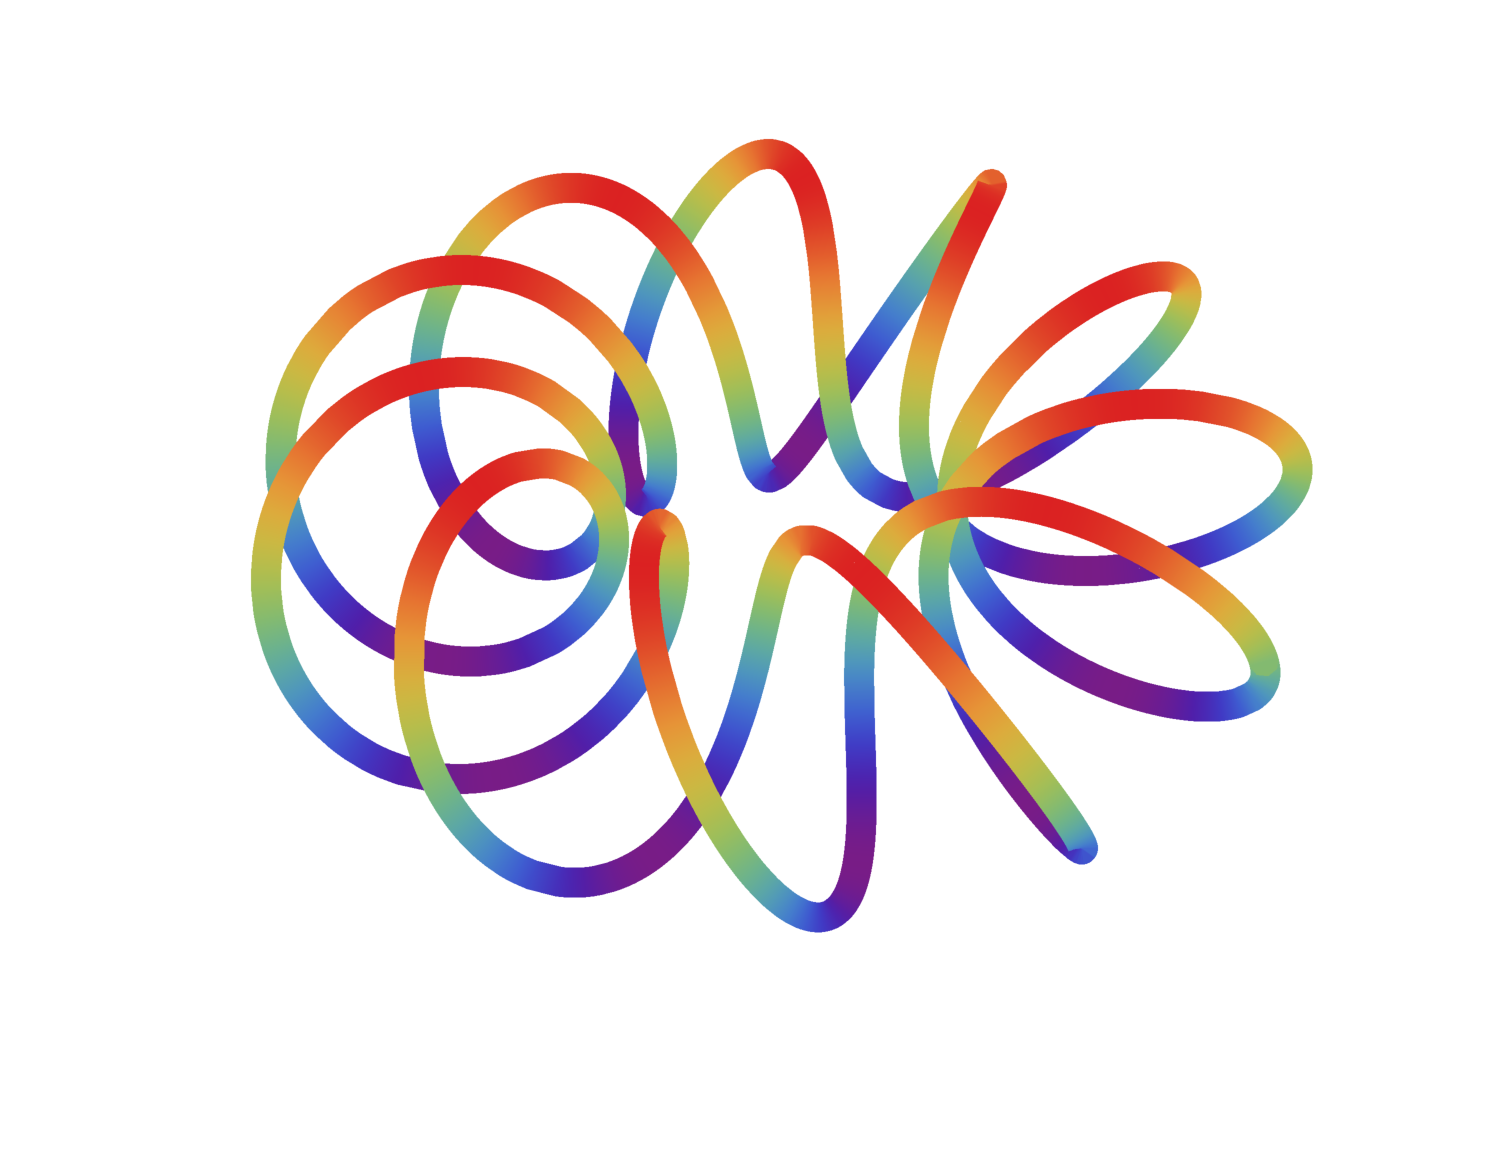
\includegraphics[width=\linewidth]{../data/torus-p2-q11.pdf}
        \subcaption{$p = 2, q = 11$}
    \end{minipage}
    \begin{minipage}[b]{.3\linewidth}
        \centering
        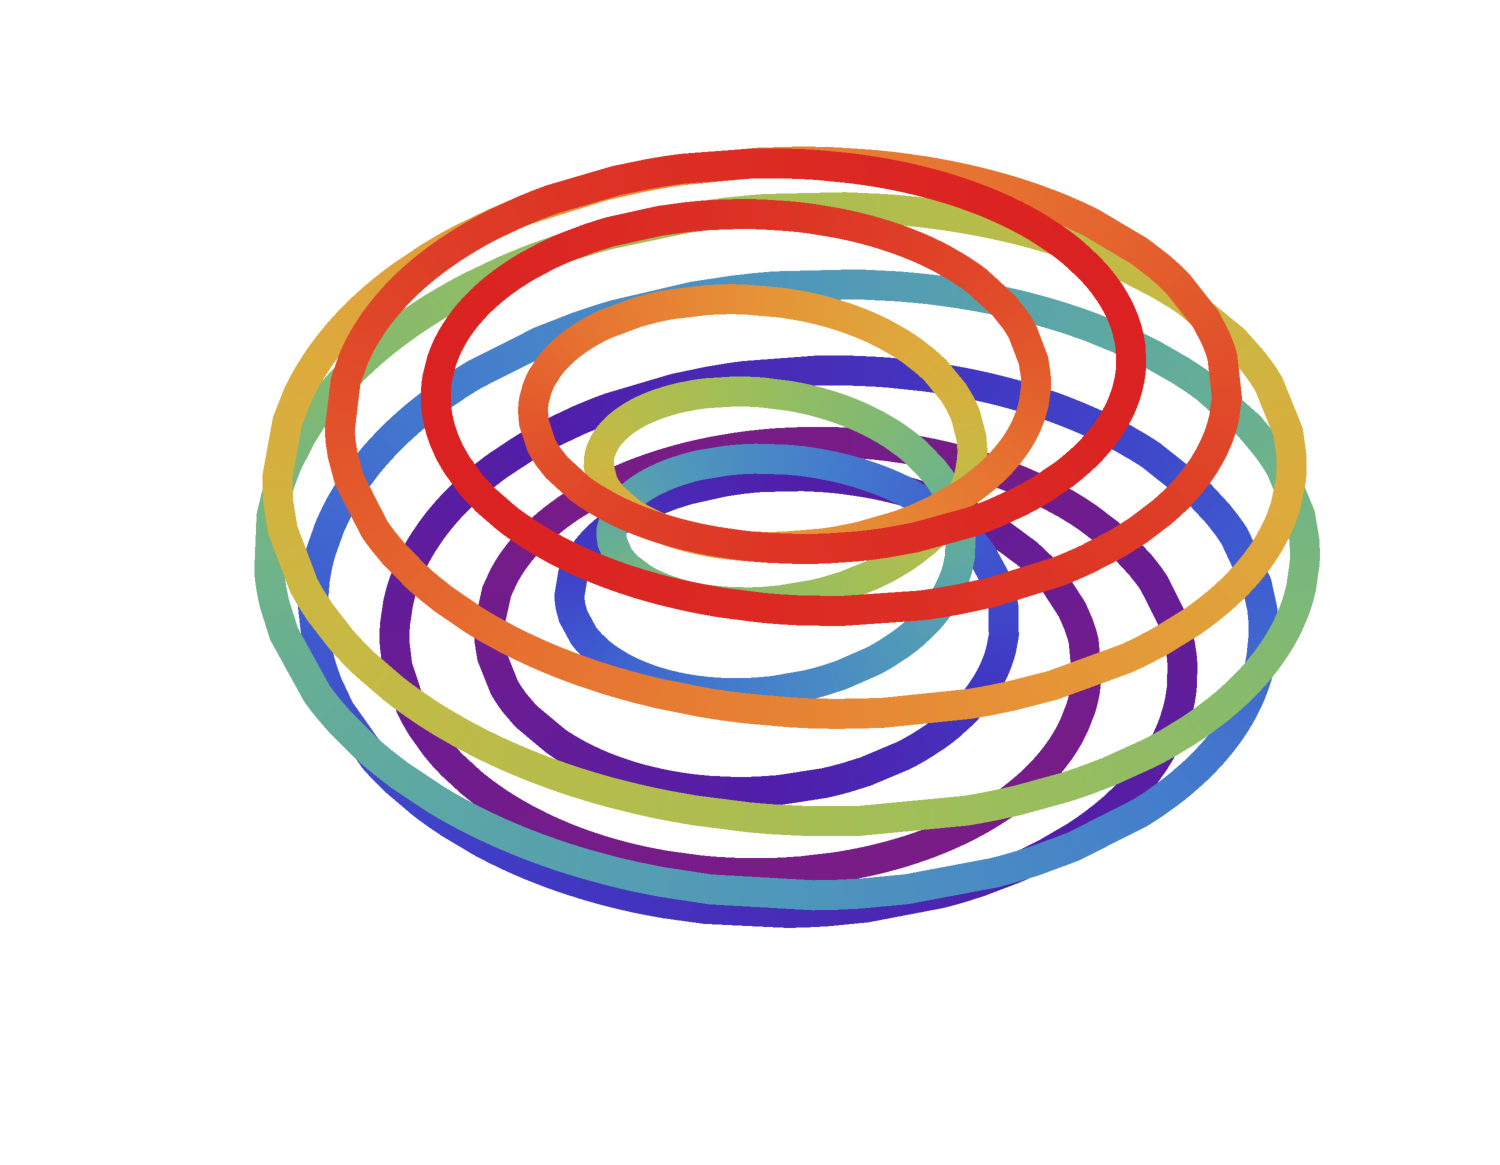
\includegraphics[width=\linewidth]{../data/torus-p11-q2.pdf}
        \subcaption{$p = 11, q = 2$}
    \end{minipage}
\end{figure}

Okazuje się, że innych obiektów już nie ma.

\begin{proposition}
    Jeśli żadna ze składowych splotu torusowego nie jest postaci $K_{0, 0}$ lub $K_{1, 0}$, to splot ten jest równoważny ze splotem $K_{q, r}$ dla pewnych $q, r$.
    Największy wspólny dzielnik indeksów $q, r$ jest jednocześnie liczbą składowych splotu.
\end{proposition}

%Węzeł ten leży na torusie $(r - 2)^2 + z^2 = 1$.
% p = 5;
% q = 3;
% ParametricPlot3D[
% {
% Cos [2 Pi p t] (2 + Cos[2 Pi q t]),
% (2 + Cos[2 Pi q t]) Sin[2 Pi p t],
% -Sin[2 Pi q t]},
% {t, 0, 1},
% ColorFunction -> "Rainbow",
% PlotStyle -> Thickness[0.02],
% Boxed -> False,
% Axes -> False
% ]

Siedem węzłów z tabeli na końcu książki to węzły torusowe.
Są to niewęzeł, $3_1 = T_{3,2}$, $5_1 = T_{5,2}$, $7_1 = T_{7,2}$, $8_{19} = T_{4,3}$, $9_1 = T_{9,2}$ oraz $10_{124} = T_{5, 3}$.

\begin{proposition}
    Ustalmy względnie pierwsze $q, r$ takie, że $|q|, |r| \ge 2$.
    Splot $K(q, r)$ jest równoważny z~odwrotnym do niego splotem $K(-q, -r)$.
\end{proposition}

Sploty $K(q, r)$ oraz $K(r, q)$ również są równoważne.
Murasugi prezentuje w~książce \cite{murasugi96} przyjemny dowód opierający się na następującym lemacie:
Sfera $S^3$ powstaje z~powierzchni dwóch węzłów trywialnych z~wnętrzem ($D^2 \times S^1$) przez wzajemne sklejenie południka i~równoleżnika z~równoleżnikiem i~południkiem.

% {\color{red} Longitude, meridian -- ustalić słownictwo}

Macierze Seiferta $M$ mają nieskomplikowaną blokową budowę, która może posłużyć do znalezienia wielomianu Alexandera (wzorem $\Delta = \det (M - tM^t)$).
Rachunki są nieco uciążliwe.

\begin{proposition}
    Wielomianem Alexandera splotu torusowego $K(q, r) \neq K(0,0)$ o~$d$ składowych jest
    \[
        \Delta_{q, r}(t) = (-1)^{d-1} \frac{(1-t)(1 - t^{qr/d})^d}{(1-t^q)(1-t^r)} \left/t^{(q-1)(r-1)/2}\right. .
    \]
\end{proposition}

\begin{proof}
    Macierzą Seiferta węzła torusowego $K(q,r)$ jest macierz
    \[
        M = \begin{bmatrix}
            B & & & & \\
            -B & B & & & \\
            & \ddots & \ddots & & \\
            & & \ddots & B & \\
            & & & -B & B
        \end{bmatrix}
    \]
    złożona z~$(r-1)^2$ bloków o~wymiarach $(q-1) \times (q-1)$:
    \[
        B \begin{bmatrix}
            -1 & & & & \\
            1 & -1 & & & \\
            & 1 & \ddots & & \\
            & & \ddots & -1 & \\
            & & & 1 & -1
        \end{bmatrix} \qedhere
    \]
\end{proof}

Znajomość wielomianu Alexandera wystarcza na szczęście do podania pełnej klasyfikacji węzłów torusowych bez uciążliwego dowodu.

\begin{proposition}
    Węzły torusowe $K(q, r)$, $K(p, s)$ są równoważne wtedy i~tylko wtedy, gdy $\{q, r\} = \{p, s\}$ lub $\{q, r\} = \{-p, -s\}$.
\end{proposition}

\begin{proof}
    Ograniczymy się do przypadku, gdy $p, q, r, s \ge 2$.
    Tylko jedna implikacja wymaga dowodu, w~prawo.
    Bez straty ogólności załóżmy więc, że $q > r$, $p > s$.
    Skoro węzły $K(q, r)$ i~$K(p,s)$ są równoważne, to porównanie najwyższych współczynników w~ich wielomianach Alexandera daje równość $(q-1)(r-1) = (p-1)(s-1)$.
    Wymnożenie wszystkiego prowadzi do czterech przypadków: $s = r$, $s = ps$, $qr = r$, $qr = ps$, z~których dwa środkowe nie mogą zachodzić (gdyż $p, q > 1$).
    Z czwartego wynika, że $qr \le s < ps$, czyli sprzeczność.
\end{proof}

Podamy teraz wartości całkowitoliczbowych niezmienników dla węzłów torusowych przy założeniu, że $q$ lub $r$ nie jest zerem.
Nietrywialne węzły torusowe są pierwsze i~odwracalne, ale mają niezerową sygnaturę, więc nie są chiralne (wiedział to Schreier w 1924: ,,Über die Gruppen $A^a B^b = 1$'').

\begin{proposition}
    Węzeł torusowy $K(q, r)$ ma okres $|q|$ oraz $|r|$.
\end{proposition}

\begin{proposition}
    Dla $q, r > 0$ zdefiniujmy wielkość $\sigma(q, r) = - \sigma(K_{q, r})$.
    Wtedy, jeśli
    \begin{itemize}[leftmargin=*]
    \itemsep0em
        \item $2r < q$ i~$r$ jest parzyste, to $\sigma(q, r) = \sigma(q-2r, r) + r^2$.
        \item $2r < q$ i~$r$ jest nieparzyste, to $\sigma(q, r) = \sigma(q-2r, r) + r^2 - 1$.
        \item $\sigma(2r, r) = r^2 - 1$.
        \item jeśli $r \le q < 2r$ i~$r$ jest parzyste, to $\sigma(q, r) + \sigma(2r-q, r) = r^2-1$.
        \item jeśli $r \le q < 2r$ i~$r$ jest nieparzyste, to $\sigma(q, r) + \sigma(2r-q, r) = r^2-2$.
    \end{itemize}
    Co więcej, $\sigma(q, r) = \sigma(r, q)$, $\sigma(q, 1) = 0$, $\sigma(q, 2) = q-1$.
\end{proposition}

Dowód zawiera praca \cite{litherland81}.
Borodzik niedawno przyjrzał się dokładniej sygnaturom węzłów torusowych.
W pracy \cite{borodzik10} napisanej z K. Oleszkiewiczem pokazał, że nie istnieje wymierna funkcja $R(p, q)$, która pokrywałaby się z sygnaturą węzła torusowego $T_{p, q}$ dla wszystkich względnie pierwszych i nieparzystych $p$ oraz $q$.
Uwaga: definicja funkcji $s$ z \cite{borodzik10} zawiera złośliwą literówkę.

\begin{proposition}
    Niech $p, q$ będą względnie pierwszymi liczbami, zaś $C \in [0, 1)$ stałą taką, że $Cpq$ nie jest liczbą całkowitą.
    Przyjmijmy $z = \exp (2 \pi i C)$ i zdefinujmy pomocnicze funkcje: niech $\{x\} = x - \lfloor x \rfloor$ oznacza część ułamkową, zaś
    \begin{equation}
        \langle x \rangle = \begin{cases}
            0 & \text{dla } x \in \Z \\
            \{x\} - 1/2 & \text{dla } x \not \in \Z
        \end{cases}
    \end{equation}
    funkcję piłę.
    Dalej, określmy sumę Dedekinda
    \begin{equation}
        s(p, q, x) = \sum_{j = 0}^{q-1} \left\langle \frac {j}{q} \right\rangle \left\langle \frac {jp}{q} + x \right\rangle.
    \end{equation}
    Przy tych oznaczeniach, sygnatura węzła $(p, q)$-torusowego wyznacza się wzorem
    \begin{align}
        \sigma(z) & = \frac{1}{3pq} \left (p^2 + q^2 + 6 \langle Cpq \rangle^2 - \frac {1}{2} \right)  + 2(C^2 - C) pq + (2-4C) \langle Cpq \rangle + {} \\
        & - 2s(p, q, Cp) - 2s(q, p, Cq) - 2s(p, q, p-pC) - 2s(q, p, q-qC). \nonumber
    \end{align}
\end{proposition}

\begin{corollary}
    Jeśli $p, q$ są nieparzyste i względnie pierwsze, to
    \begin{equation}
        \sigma(T_{p,q}) = \frac{1}{6pq} + \frac{2p}{3q} + \frac{2q}{3p} - \frac{pq}{2} - 4(s(2p, q, 0) + s(2q, p, 0)) - 1.
    \end{equation}
\end{corollary}

\begin{corollary}
    Jeśli $p$ jest nieparzyste, zaś $q > 2$ parzyste, to
    \begin{equation}
        \sigma(T_{p,q}) = - \frac{pq}{2} + 4s(2p, q, 0) - 8s(p, q, 0) + 1.
    \end{equation}
\end{corollary}

\begin{proposition}[Murasugi, 1991]
    Mamy $cr(K_{q,r}) = \min\{|q|(|r| -1), |r|(|q|-1)\}$.
\end{proposition}

Wyznaczenie indeksu rozwiązującego było dużo trudniejsze.
Murasugi pisze w~książce \cite{murasugi96}, że mamy nierówność
\[
    u(K(q, r)) \le \frac 12 (q-1)(r-1),
\]
z równością dla względnie pierwszych $q, r > 0$.
Hipoteza Milnora głosiła, że w~rzeczywistości równość zachodzi zawsze.
Dowód został odnaleziony w~latach 1993-1995 przy użyciu tzw. \emph{gauge theory} (działu teorii pola, gdzie lagranżjan jest niezmienniczy względem grup Liego lokalnych transformacji...).
Patrz prace \cite{kronheimer93} oraz \cite{kronheimer95}.

\begin{proposition}[Kronheimer, Mrówka] \label{torus_unknotting}
    Dla względnie pierwszych $q, r > 0$ mamy
    \[
        u(K(q, r)) = \frac 12 (q-1)(r-1),
    \]
\end{proposition}

Genus pokrywa się z~liczbą gordyjską dla węzłów (czyli względnie pierwszych $q, r$).

\begin{proposition} \label{torus_bridge}
    Indeksem mostowym węzła $K_{q,r}$ jest mniejsza z~liczb $|q|, |r|$.
\end{proposition}

\begin{proposition}
    Mamy $\bracket{K_{2, n}} = A \bracket{K_{2,n-1}} + (-1)^{n-1} A^{2-3n}$
    oraz $\bracket{K_{2,1}} = -A^3$.
\end{proposition}

\begin{proposition}
    Wielomianem Jonesa węzła $(m, n)$-torusowego jest
    \[
        V(t) = \frac {t^{(m-1)(n-1):2}}{1-t^2} \cdot (1 - t^{m+1} - t^{n+1} + t^{m+n}).
    \]
\end{proposition}

Murasugi i~Neuwirth w~1961 dla węzłów alternujących,
zaś Burde z~Zieschangiem w~1965 pokazali, że nietrywialny węzeł,
którego grupa ma nietrywialne centrum, jest torusowy.

\begin{proposition}
    Wielomianem Alexandera węzła $(p,q)$-torusowego jest
    \[
         \Delta(T_{p,q}) = \frac{(t^{pq}-1)(t-1)}{(t^p-1)(t^q-1)}.
    \]
\end{proposition}

\begin{proof}
    Przypadek $p = 2$ wymaga prostego rozumowania indukcyjnego.
    Samo ćwiczenie pojawia się w~wielu podręcznikach topologii.
    Pełny dowód można znaleźć w~przykładzie 9.15 książki ,,Knots'' Burdego oraz Zieschanga.
    Inne podejście, tak zwaną formułę Seiferta-Torresa, prezentuje przeglądowa praca Turaewa ,,Reidemeister torsion in knot theory'', 119-182.
\end{proof}

\begin{corollary}
    Wielomian Alexandera odróżnia od siebie węzły $(2,n)$-torusowe.
\end{corollary}

\begin{proof}
    Mamy $\Delta(T_{2,n}) = (t^n+1) / (t+1)$, więc $\deg \Delta (T_{2,n}) = n - 1$.
\end{proof}

% Koniec sekcji Węzły torusowe
